% Use only LaTeX2e, calling the article.cls class and 12-point type.

\documentclass[12pt]{article}

% Users of the {thebibliography} environment or BibTeX should use the
% scicite.sty package, downloadable from *Science* at
% www.sciencemag.org/about/authors/prep/TeX_help/ .
% This package should properly format in-text
% reference calls and reference-list numbers.

\usepackage{scicite}
\usepackage{times}
\usepackage{graphicx}
\usepackage{lineno}
\usepackage{longtable}
%\usepackage{multicolumn}
\usepackage[skip=2pt,font=normalsize]{caption}
\usepackage[LGRgreek]{mathastext}
\usepackage{multirow}
\usepackage[
  breaklinks=true,
  colorlinks=true,
  linkcolor=blue,anchorcolor=blue,
  citecolor=blue,filecolor=blue,
  menucolor=blue,pagecolor=blue,
  urlcolor=blue]{hyperref}

% The following parameters seem to provide a reasonable page setup.

\topmargin 0.0cm
\oddsidemargin 0.2cm
\textwidth 16.5cm 
\textheight 21cm
\footskip 1.0cm


%The next command sets up an environment for the abstract to your paper.

\newenvironment{sciabstract}{%
\begin{quote} \bf}
{\end{quote}}

\usepackage{array}
\newcolumntype{L}[1]{>{\raggedright\let\newline\\\arraybackslash\hspace{0pt}}m{#1}}
\newcolumntype{C}[1]{>{\centering\let\newline\\\arraybackslash\hspace{0pt}}m{#1}}
\newcolumntype{R}[1]{>{\raggedleft\let\newline\\\arraybackslash\hspace{0pt}}m{#1}}

% If your reference list includes text notes as well as references,
% include the following line; otherwise, comment it out.

%\renewcommand\refname{References and Notes}

% The following lines set up an environment for the last note in the
% reference list, which commonly includes acknowledgments of funding,
% help, etc.  It's intended for users of BibTeX or the {thebibliography}
% environment.  Users who are hand-coding their references at the end
% using a list environment such as {enumerate} can simply add another
% item at the end, and it will be numbered automatically.

\newcounter{lastnote}
\newenvironment{scilastnote}{%
\setcounter{lastnote}{\value{enumiv}}%
\addtocounter{lastnote}{+1}%
\begin{list}%
{\arabic{lastnote}.}
{\setlength{\leftmargin}{.22in}}
{\setlength{\labelsep}{.5em}}}
{\end{list}}


% Include your paper's title here

%%%%%%%%%%%%%%%%% END OF PREAMBLE %%%%%%%%%%%%%%%%

\newcommand{\beginsupplement}{%
        \setcounter{table}{0}
        \renewcommand{\thetable}{S\arabic{table}}%
        \setcounter{figure}{0}
        \renewcommand{\thefigure}{S\arabic{figure}}%
     }


\begin{document} 
\beginsupplement

\linenumbers
\baselineskip24pt

\section*{Supplementary Information}% Make the title.

The following text provides additional information on this study's Methods and Results.  The full manuscript, data, and code for all calculations are available on an accompanying \href{https://github.com/agroimpacts/ecoscales}{github repository}. \textbf{Note to editors and reviewers: this repository is currently private, but will be made public upon acceptance of manuscript. In the interim, the entire project folder can be downloaded from the following \href{https://www.dropbox.com/sh/1l9em6p0wyabwr3/AADhCpFvqjv6y7VbL5tgB3Iqa?dl=0}{link}.}

\subsection*{Methods}% Make the title.
\vspace{-4pt}
%\maketitle 
\subsubsection*{Paper selection}
\vspace{-10pt}
We used the 2012 Web of Science impact factors to select the highest ranked ecology-themed journals that published studies with an observational component, excluding journals devoted to reviews, meta-analyses, laboratory, cellular, or experimental studies.  To select a representative sample of recent ecology studies, we downloaded the metadata for all papers published in the selected journals (Table S1) between 2004 and 2014. Our study involved six different observers (those reviewing the papers to extract the observational scales), each of whom was given a randomly selected batch of 500 titles.  A separate set of 20 papers was also randomly selected, and this set was given to all observers to review independently, in order to 1) calibrate the interpretations and extraction of scale-related information between observers, and 2) to estimate between-observer variance.  

\centerline{
%\hspace{1cm} 
\parbox{11cm}{\noindent Table 1. The selected journals and their 2012 impact factors.}
}
\vspace{-12pt}
%\begin{longtable}[h]
\begin{longtable}{lr}
%\centering
%\caption{The selected journals and their 2012 impact factors.}\\
%\centering
%\begin{tabular}{lr}
  \hline
\textbf{Journal} & \textbf{Impact Factor} \\
\hline
\endhead 
  \hline
Ecology Letters & 17.95 \\ 
  Ecological Monographs & 8.09 \\ 
  Frontiers In Ecology And The Environment & 7.62 \\ 
  Global Ecology And Biogeography & 7.22 \\ 
  Global Change Biology & 6.91 \\ 
  Diversity And Distributions & 6.12 \\ 
  Methods In Ecology And Evolution & 5.92 \\ 
  Proceedings Of The Royal Society B-biological Sciences & 5.68 \\ 
  Journal Of Ecology & 5.43 \\ 
  Ecology & 5.17 \\ 
  Ecography & 5.12 \\ 
  Journal Of Biogeography & 4.86 \\ 
  Functional Ecology & 4.86 \\ 
  Journal Of Animal Ecology & 4.84 \\ 
  Journal Of Applied Ecology & 4.74 \\ 
  American Naturalist & 4.55 \\ 
  Conservation Biology & 4.36 \\ 
  Ecological Applications & 3.81 \\ 
  Biological Conservation & 3.79 \\ 
  Biogeosciences & 3.75 \\ 
  Bulletin Of The American Museum Of Natural History & 3.48 \\ 
  Biology Letters & 3.35 \\ 
  Oikos & 3.32 \\ 
  Behavioral Ecology & 3.22 \\ 
  Ecosystems & 3.17 \\ 
  Advances In Ecological Research & 3.08 \\ 
  Oecologia & 3.01 \\ 
  Landscape Ecology & 2.90 \\ 
  Agriculture Ecosystems \& Environment & 2.86 \\ 
  Ecological Economics & 2.85 \\ 
   \hline
%\end{tabular}
\end{longtable}
% Place your abstract within the special {sciabstract} environment.

\subsubsection*{Estimating observational scales}
\vspace{-10pt}

Each observer first reviewed the papers in the calibration set, and then commenced reviewing papers in their individual random draws, beginning at the top of the list and then proceeding until at least 20 eligible papers describing ecological observations were reviewed. In cases where the reviewed papers used observations that were described in another publication, we reviewed those source papers in order to extract the observational dimensions. We excluded papers that were opinion or perspectives pieces (unless they presented or used existing observational data), theoretical studies based on generated data, or those which were entirely based on experimental manipulations. We left out the latter category because our intent was to evaluate the domains for observations of natural systems, and we wanted to avoid the bias that would be imposed by the relatively narrow spatial and temporal scales of experiments \cite{kareiva_spatial_1988,tilman_global_2011}.  A bibliography of the reviewed papers follows the References and Notes section below. 

We recorded six primary dimensions of ecological observations, three related to space and three related to time.  The space-related dimensions were resolution, extent, and actual extent. Here extent was primarily defined as the area falling within a perimeter defined by the outermost spatial replicates, while actual extent was defined as the summed area of all sample plots (i.e. N * resolution, where N is the number of spatial replicates, which we also recorded), or the area that ecologists observe in practice. In assessing spatial scales, our analysis only considered the Cartesian plane. We did not calculate the z, or depth, dimension, although this dimension is of greater importance for certain sub-disciplines of ecology (e.g. depth profiles in marine ecology). In some cases (primarily paleoecological studies), values extracted from the z-dimension provided temporal information that was used to calculate both the interval and the duration of the observation.  

For time dimensions, we extracted information related to interval, duration, and actual duration. Duration was defined as the time between the first and last temporal replicate, whereas actual duration quantifies the amount of time spent observing a particular location, which we calculated by multiplying sampling duration (the time spent collecting a single temporal replicate) by the number of temporal replicates.  

A full definition of all dimensions and how they were recorded is contained within the answers to the list of questions below. This set of Frequently Asked Questions (FAQ) was provided to each observer for initial study and reference, in order to ensure methodological consistency (see next section).  

%To record the spatio-temporal dimensions of ecological observations, we considered the observational scales to be those at which a total measurement of the feature(s) of interest was made, rather than the scales that might be represented by the observations.  As an example, if a paper reported data on plant species diversity collected using 10 1 m$^2$ sub-plots randomly placed within a larger plot of 100 m$^2$, of which 10 were placed, we recorded 1 m$^2$ as the spatial resolution and 100 m$^2$ as the total extent of the observation. 

%While the 10 sub-plots might be representative of diversity at larger scales (e.g. the particular plant community), that relationship depends both on sample design (number of replicates, placement, grain/resolution) and the properties of the ecosystem \cite{underwood_experiments_1997,palmer_scale_1994, cao_comparison_2002}. Most studies also did not quantify the broader scales represented by their observations, nor did they report dimensions that would allow these to be independently estimated, such as the maximum distance between sample plots, which could have been used to estimate the spatial extent represented by the sample \cite{palmer_scale_1994}.

%Similarly, we did not try to quantify the extent to which values of individual observations (e.g. a single plot) of an ecological feature might be correlated with spatially or temporally adjacent values.  Autocorrelation is common to most ecological phenomena \cite{legendre_spatial_1993,collins_method_2000-1}, and it means that an observation can be representative of the properties within a broader area or time around the point at which it is taken. For example, soil properties are typically measured by analysis of soil cores collected using an augur. The two-dimensional resolution of this measurement is equal to the area of the augur, but the measured soil properties are likely to be very similar, if not identical, to those found in the soil within a radius of at least a few to several hundreds of meters around the core location. However, the distance and strength of this correlation can vary substantially according to the ecological features being observed, and such correlation lengths were reported in almost no studies. Attempting to estimate these lengths, and add them to actual observations scales, would have added further uncertainty to estimates. Moreover, this concern only applies to spatially and temporally discontinuous (or discontiguous) observations, and since many of observations are collected using techniques that permit continuous measurements (e.g. weather data over time or satellite images over space), we elected to use a consistent standard for estimating dimensions. 

%Furthermore quantifying the actual domains of observation is important because highly dynamic spatial and temporal processes, such as the population ecology of riverine fish \cite{fausch_landscapes_2002} or the evolution of wildfires \cite{clements_observing_2007}, may require continuous observation to properly measure, and can vary substantially in the space or time between observations.  

\noindent\underline{\textbf{General:}}
\def\Hitem{\item [Q\stepcounter{enumi}\arabic{enumi}.]} 
\def\Hsubitem{\item [Q\arabic{enumi}.\arabic{enumi}.]} 
\vspace{-0.5cm}
\begin{enumerate}
  \Hitem \emph{\textbf{What are the general inclusion/exclusion criteria for studies?}} Studies should be excluded from this analysis if they are: 1) opinion/perspectives pieces; 2) book reviews; 3) model-only studies, particularly theoretical models, which are not developed or tested against observed data; 4) if they are experimental manipulations (but if there is a study that has a mix of observational and experimental, record the observational treatments and exclude the manipulated treatments).
  
  \Hitem \emph{\textbf{What are the standard categories to be used for defining �Study type�?}} Define study type according to the following categories: Remote sensing, passive/automated data collection, other geographic data (e.g. non-remotely sensed GIS data), field/direct observation, or paleo-reconstruction (tree rings, charcoal cores, etc).

  \Hitem \emph{\textbf{What happens when the study draws on a separately published dataset as a key part of the methods?}} Track down the study describing the paper, and then record the DOI of that paper/those papers.
  
  \Hitem \emph{\textbf{What is the best unique identifier of a study I am reviewing?}} The DOI! 
  
  \Hitem \emph{\textbf{What do I record for a time or space scale when it is not clearly reported in the paper, or when I am unsure? For example, in a paleo-ecological study looking at historical charcoal deposition, sediment cores were extracted from lakes, which the authors report as the number of samples. However, it is unclear how many sediment cores were drawn from each lake, and it is these which should be the number of spatial replicates.}} For these sorts of issues, we record that the scale in question is uncertain, and then your best estimate of the measure (e.g. you might assume that only 1 core was made per lake).

\hspace{-1cm}\underline{\textbf{Temporal scales:}}
\vspace{-0.5cm} 
   \Hitem \emph{\textbf{What is interval, and how do we record it?}} Interval is the time that elapsed between repeated observations of the same point in space or individual organism. In many cases, observations will only be made one time--list a value of 0 for these.  
  \Hitem \emph{\textbf{What is sampling duration, and how do we record it?}} How long an individual observation of an individual point in space took to make. Sampling duration multiplied by the number of repeats observations is used to calculate study duration. Often this value will not be reported, so you will have to use your best judgement, based on your knowledge of ecological methods, to approximate the sampling duration. For example, for a field based method with intensive plot methods, if you can't estimate a plausible sampling duration, assign a token 1 day. For remote sensing observations you can assume one second (although the observations are effectively instantaneous).  
   \Hitem \emph{\textbf{What is duration, and how do we estimate it?}} The duration is the total period of time over which the phenomenon of interest was observed. More specifically, in the case of repeated observations, this is the total time that elapsed between the first and last observations at a given point in space (or of the same individual organism or community). For once-off (unreplicated) observations, this time is equivalent to the sample duration. However, there may be cases where once-off observations may have a longer duration than the sample duration.  For example, consider a study that counts occurrences of pollinators over three years, using transects that are located in different locations within the broader study area during each year \cite{rollin_differences_2013}. The observations are therefore not strictly temporally replicated, but the authors control for year of collection in their subsequent analysis to avoid confounding effects.  In this case, we can consider the effective duration to be three years, as the temporal information is encoded in the analysis. 
  \Hitem \emph{\textbf{What is \emph{actual duration}, and how do we calculate it?}} The actual duration is the integral of sampling duration, or the time spent making one observation of the phenomenon in question. To clarify, actual duration is the total time spent sampling/observing a single point in space--not the span of time between first and last sample (duration), nor the integral of time spent in observing all spatial replicates. 
  \Hitem \emph{\textbf{Should actual duration be the total time spent sampling all sites or the amount of time spent sampling per site (e.g. for 5 minute point counts of birds at 10 sites each repeated twice, should we enter 100 minutes (5 minutes X 2 repeats X 10 sites) or 10 minutes (5 minutes X 2 repeats) for duration)?}} As stated above, actual duration is the total spent observing a single point in space, so in this case that would be 10 minutes (then converted to days, so 10 / (60 * 24))).
  \Hitem \emph{\textbf{How do we record duration and actual duration when there are no repeat observations?}} In these cases, study duration is equal to sampling duration. 
   \Hitem \emph{\textbf{How do I record interval in cases where the interval is inconsistent?  For example, in a study were observations were observations were repeated in 1979, 1980, 1981, 1984, 2007, 2009?}} Find the time between each successive period, and then take the average of that (remember to convert to days!). If there are two or more sets of unevenly spaced days for each site/plot/measurement being taken in the study, then find the average interval for each, and average the averages.  
    \Hitem \emph{\textbf{How do you determine the interval for paleo-reconstructions?}} Use the minimum estimate for dating precision as the estimate of time between samples (e.g. 50 years in the study of European charcoal deposits DOI:10.1111/geb.12090). 
    \Hitem \emph{\textbf{How do you determine the sample duration (our third time category) for paleo-reconstructions?}} Similar to the previous question, the sampling duration is also the same as the minimum estimate of dating precision. The logic behind this is that in such cases, where a sediment or tree core or similar measurement is being collected, this effectively represents a continuous ``observation'', and the value associated with the minimum (or other reported) interval is typically an average (or another summary statistic like the maximum) of the amount accumulated. 
    \Hitem \emph{\textbf{What about intervals and durations for instrument-collected, or automatically-collected, observations?}} These are often similar in essence to the paleo-reconstruction case. Take the minimum temperature or daily rainfall recorded at a weather station, which require constant observation over 24 hours to report. In such cases, the interval and sampling duration are both 24 hours. On the other hand, automated logging systems will provide a series of high frequency observations that are collected instantaneously. In these cases the sampling duration should be a token one second (to keep consistent with remote sensing [Q7]), and the interval should be the period between successive instantaneous measurements. 
    \Hitem \emph{\textbf{How do you treat interval for a case where repeated samples are taken during a season, across several seasons (e.g.``we performed repeat bird counts every 10 days between March and June of 2005, 2006, and 2008'')?}} Since the sampling is focused on seasons, and presumably some season-specific phenomenon (e.g. breeding behavior), the reported values should be pegged to the season, not averaged across the duration (the start and end dates of the study). So in this example, it would be 10 days.  

\hspace{-1cm}\underline{\textbf{Spatial scales:}}
  \Hitem \emph{\textbf{What is resolution, and how do I record it?}} This is the finest scale at which a complete measurement of every unit of the quantity of interest is recorded.  For example, if the measurement in question is a tree stem count, the resolution is determined by the size of the plot used to record every tree stem. Taking this example further, let's say a study reports a plot size of 100 x 100 m, but then goes on to report that they counted stems within a single 1 m wide transect within this larger plot.  In this case, the plot resolution is in fact 100 m x 1 m, or 100 m$^2$ (sampling resolution should be reported in m$^2$).  In another example, if the reported plot size was 20 x 20 m, but the authors in fact only measured a random selection of, say, grass stems on which they counted aphids within those plots, then use an estimate of the area of the grass stem as the sampling resolution \cite{gagic_agricultural_2012}.  
 
  \Hitem \emph{\textbf{What is extent, and how do I record it?}} Extent is defined as the total area enclosed within a perimeter defined by the outermost spatial replicates, divided by 10,000 to convert to hectares. For studies in which spatial replicates are not spatially contiguous, this means the area of the minimum polygon bounding all spatial replicates. To calculate the effective survey extent, use the area of the study area/region given in the paper; when the area is not given, but when the survey region is given by name (e.g., Joshua Tree National Park or United States), look up the area through an online search and convert to hectares, provided the observations were collected throughout the named survey region. When the area is not named, but a map is given (or if the area is named and the map of replicates shows that the replicates were located in a smaller area of the named region), use an appropriate digitizing platform with a suitable map-providing backend (e.g. Google Earth Pro, QGIS with OpenLayers plugin) to navigate to the region and delineate a minimum convex polygon surrounding the replicates (plots/transects/other sampling units) to calculate the area in hectares. There is an exception to this rule, however, for studies that focus on features that are clearly distinct and functionally isolated from their surroundings. Examples of such cases might be mangrove forests patches within in a coastal National Park, or populations of a rare species confined to three disjunct protected areas. In these cases, the extent will be the summed area of the sampled units (the summed area of sampled mangrove stands, and the summed areas of the three protected areas). In other words, try to delineate the focal portions and not the larger survey region.
  
For spatially contiguous studies (e.g. those based on satellite imagery), the extent is the total area covered by the imagery (in such cases, extent equals actual extent), but only record the area of imagery analyzed by the authors (e.g. if the study area required four Landsat scenes to cover, but covered only the inner quarter of each image, report the extent as the summed area of the four quarters). However, if spatially contiguous studies only use a sub-sample of pixels, extent is the area of the polygon enclosing the outermost pixels (calculated following the methods above).

For studies that record individual, mobile organisms as the units of observation, use the minimum polygon surrounding the outermost observations of the complete space-time dataset (i.e. observations from all individuals and times) to define extent.

  \Hitem \emph{\textbf{What is \emph{actual extent}, and how do I record it?}}  Actual extent is the sampling resolution multiplied by the number of spatial replicates, divided by 10,000 to convert to hectares. For studies in which the spatial replicates are not spatially contiguous (as with most field-based studies), this means resolution (see Q17) multiplied by number of plots. For spatially contiguous studies (e.g., those based on remote sensing imagery), it should be the total area covered by the imagery, i.e., pixel resolution multiplied by the number of pixels. However, as with extent, only record the area analyzed by the authors. If they used a sub-sample of pixels, the actual extent is the number of those pixels multiplied by pixel resolution. 
  
%But I'm noticing now that this isn't updated to include how to handle when the study unit is animals. I guess we could just add a sentence saying that the effective extent is the surface area of an average-sized individual of the animal species, or something along those lines. Let me know what you think.

  
  
%  Broadly defined, study extent is the sampling resolution multiplied by the number of spatial replicates, divided by 10,000 to convert to hectares. For studies in which the spatial replicates are not spatially contiguous (as with most field-based studies), this means plot resolution (see Q16) multiplied by number of plots. For spatially contiguous studies (e.g. those based on remote sensing imagery), it should be the total area covered by the imagery, i.e. pixel resolution multiplied by the number of pixels. However, only record the area analyzed by the authors. If they used a sub-sample of pixels, extent is the number of those pixels a multiplied by pixel resolution. 

  \Hitem \emph{\textbf{How do you determine resolution for paleo-reconstructions and other approaches where a sampling method is presumed to draw from a larger area (e.g. mammal traps, mist nets, etc)?}}  For sampling resolution, estimate the size of the sample actually taken, rather than the assumed catchment/shed area of the sample (e.g. the area of the corer used to take a sediment sample, rather than an estimate of the area that that sample is assumed to draw from), and then indicate that the plot resolution was uncertain. Related to this, you may also have to estimate the number of samples collected, as exemplified in a charcoal study of Europe where the number of lakes sampled was provided, not the number of cores per lake \cite{molinari_exploring_2013}.  

  \Hitem \emph{\textbf{What about studies that sample individual organisms?}} If the study is making a total count of all organisms (let's say a mammal species) within a fixed plot size, or even a variable plot size from which an average plot size (and thus sampling resolution) can be estimated, then follow the procedures described in Q17. However, if the individual animals are the unit of measure (either because a sub-sample of them is being made within a defined plot, or because the observation is not contingent on being located within a plot (maybe a blood sample or body weight is being recorded, for example), then simply estimate two-dimensional area occupied by the animal as the plot resolution, and the number of sampled animals provide the spatial replicates (for calculating actual extent). Occasionally individual animals might be recorded, but within the context of some natural feature, such as a nesting site where the survival of individual chicks is the measurement of interest \cite{roche_relative_2008}. In this case, an estimate of the nest area provides the sampling resolution. In cases where individual animals are tracked using radio or GPS collars, to calculate actual extent, use the number of locational fixes as the quantity of spatial replicates and the animal's two-dimensional body area. If the number of GPS points is not given, the number of fixes can be estimated from the duration during which individuals were collared and the recording interval.

\end{enumerate}

\subsubsection*{Calibration and consistency}
\vspace{-10pt}
Most studies did not explicitly report values for all the assessed scales, and thus interpretation and judgement had to be applied to develop reasonable estimates for their values. The FAQ provided the protocol we followed, and was initially developed following consultation between observers prior to the commencement of review. We conducted an iterative process of calibration to ensure consistency and reliability of estimates. First, we used the calibration set to calculate between-observer variability with respect to paper selection/rejection and the estimation of scales.  Based on this, the lead author reviewed individual records in each observer's calibration set, flagged values where the estimation procedure departed from the protocol, and returned these to observers for re-estimation, without providing an estimate of the actual value. Instead, the relevant section of the protocol was highlighted, and further explanation and clarifying discussion undertaken as needed. Protocol language was adjusted for clarity during this process, and new items added to cover circumstances that had not been addressed by the initial version. The variability measures (see Results) were re-calculated after each iteration.  

To ensure consistency within the main analysis, the lead author also reviewed each observer's results from their individual draw of papers and flagged values that appeared to deviate from the protocol for re-review by the observer. Re-reviewed values were re-inspected, and in some cases a secondary review of particular papers was undertaken to cross-check the estimated scales.   

\subsubsection*{Accounting for estimation uncertainty}
\vspace{-10pt}
Two major and related sources of uncertainty affected our estimation of observational scales: 1) unclear documentation of observational scales in the reviewed studies, 2) variation between observers in estimating observational scales (largely in cases where scales were not explicitly reported). We estimated and accounted for these uncertainties in several ways. First, we calculated the degree of between-observer variability based on each observer's results from reviewing the 20-paper calibration set. We calculated how well observers agreed regarding paper inclusion/exclusion, how many extractable observations there were per included paper, and what the coefficient of variation was across all observers' estimates of scale. We also recorded when observations were reported in any study (calibration set or otherwise) with an unclear or missing scale value. 

We used the between-observer coefficients of variation for each dimension as the basis for randomly perturbing the scale values for each of the 371 observations over 1000 iterations. For each observation at each iteration, we perturbed its scale value in each dimension by randomly selecting (from a uniform distribution) a percentage value p that fell between 100 + y and 100 - y, where y was the between-observer coefficient of variation (expressed as a percentage) for a given observational dimension, and multiplying that observation's scale value by that proportion. In certain cases, the perturbation resulted in values for some certain dimensions that were not physically possible (e.g. interval longer or actual duration longer than duration; actual extent larger than extent), in which case we adjusted the perturbed values for the dimension that should be the smallest to equal that of the one that should be largest (e.g. we set interval to equal the perturbed duration value). This perturbed set of observations provided a basis for estimating uncertainty within our extracted set of observational scales. 

\subsubsection*{Scale metrics}
\vspace{-10pt}
In presenting results (Fig. 1 and 2 in main text), we log-transformed (base 10) the observational scales within each of the 1000 perturbed ensemble members in order to account for the large range in scale values. We calculated histograms for the four primary observational dimensions from each of the log-transformed ensemble members, calculating the mean percentage density estimate for each bin across all 1000 histograms, as well as the upper and lower 2.5th percentile values for each bin (Fig. 1 main text).  

To reveal the densities of observations within two dimensions (Fig. 2 main text), we used the splancs package \cite{rowlingson_splancs:_1993} of R \cite{r_development_core_team_r:_2011} to calculate a kernel density estimate of the log-transformed values across all ensemble members, using a bandwidth of 1 on a 0.1 resolution image to provide a smoothed result that served to more effectively highlight domains in which ecological observations are concentrated. Bandwidths of varying resolutions were tested on kernel density estimates were tested on kernel density estimates of sampling interval versus plot resolution (see Supplementary Results section).  

To compare the differences between actual extent and extent and actual duration and duration (Fig. 3 main text) we calculated the magnitude of difference (decade) between each pair as:

\begin{equation}
decade = log_{10}(x) - log_{10}(y) = log_{10}\left(\frac{x}{y}\right)
\end{equation}

\noindent Where x is either extent or duration and y is its actual counterpart. We then evaluated how the magnitudes of difference varied with increasing values of actual extent/duration, using box plots to summarize decades within the same bins used for extent and duration (Fig. 1B and D main text). Decades were calculated for each pair for all bootstrap replicates. The whiskers in the summary box plots (Fig. 3 main text) fall slightly below 0 in some bins, even though extent and duration can never be smaller than their actual value. This is an artifact of the perturbation applied to estimated values, which in some instances caused extent/duration values to fall below their actual value. We retained these discrepancies rather than forcing such cases to zero to avoid biasing the summary statistics. 

\subsubsection*{Trends in methods and scale}
To assess the degree to which observational methods changed over the course of the 10 years worth of studies we surveyed, we calculated the percentage of observations made using remote sensing, general field methods, and automated \emph{in situ} methods, and fit a linear regression between these percentages and publication year, weighting the regression by the total number of observations in each year.  We performed the same analysis for the four primary dimensions (resolution, extent, interval, and duration) in order to assess whether there were any trends in observational scales.  

\subsubsection*{Extracting and analyzing data from earlier meta-analyses}
To compare the results of our analysis with the observational scales of earlier ecological studies, we used graph capture software\footnote{http://arohatgi.info/WebPlotDigitizer/app/} to extract the data values from Figure 6.1 in Tilman \cite{tilman_ecological_1989}, Figure 1 in Kareiva and Anderson \cite{kareiva_spatial_1988}, and Figure 2 in Porter et al \cite{porter_crop_2005}. To maintain as much comparability as possible with our inclusion criteria, we excluded experiment studies in Tilman's data, as well as the values of any studies having duration values greater than 100 years (no upper time bound was provided for these), leaving duration values for 419 (out of 623) studies. As Tilman presented duration values as a histogram, we calculated the mean duration across all studies as the weighted (by number of observations per bin) mean of bin center-point values (i.e. the weighted mean of the bin means).  We also excluded four (of 29) observation values from Porter et al's data on observational extent and frequency, which, in contrast to the other 25, were not randomly selected. Porter et al also used irregular scales for both their X (frequency) and Y (extent) axis, therefore we had to visually estimate the scale values for each data point after graphical extraction, and converted their extent values (in km) to hectares and their frequency values to intervals. Kareiva and Anderson presented resolution as plot diameters (m), which we squared to make comparable to our resolution metric. 

\subsection*{Results}
\vspace{-4pt}

\subsubsection*{Variability and consistency between observers}
\vspace{-10pt}

We assessed variability and consistency between observers along multiple dimensions. First, we assessed how reliably observers agreed with respect to selecting or rejecting papers for review, using the R's Agreement package \cite{yu_agreement:_2012} to calculate Fleiss' kappa statistic \cite{fleiss_measuring_1971}, which was 0.72 (z = 12.5, p$<$0.000), indicating substantial and significant agreement between observers \cite{landis_measurement_1977}. 

Second, we calculated the intra-class correlation coefficient \cite{bartko_intraclass_1966} to assess agreement between observers regarding the number of ecological observations that could be extracted from each paper (multiple ecological observations were reported in many studies; we listed observations as separate records if they measured different features, or more rarely, varied substantially on one or more dimensions).  The coefficient, calculated using the IRR package \cite{gamer_irr:_2012} of R, was 0.71 (F = 15.4, p$<$0.0001, 95\% confidence interval = 0.54 - 0.85)  

Finally, we calculated the coefficient of variation (CV) between observers' estimates of scales for each dimension, first across all observers' mean scale estimates, and then as the average CV among observers' estimates of each individual record (Table S2). CV values were estimated from all six observers for resolution, actual extent, and interval, from five observers (all but Choi) for duration, and from three observers (Elsen, Estes, and Treuer) for extent. The smaller numbers for duration and extent reflect that initial efforts were focused on estimating resolution, interval, and actual extent and actual duration, thus fewer observers were available to assess extent and extent. 

\subsubsection*{Between-observer coefficient of variation}
\vspace{-10pt}
We used the maximum uncertainty values for each dimension from the inter-observer variability analysis (Table S2) to determine the bounds of the random perturbations applied to each record over the 1000 iteration resample.  

\begin{table}[ht]
\captionsetup{width=1\linewidth}
\caption{Estimates of variability calculated from each observer's estimates of the spatial and temporal scales of ecological observations reported within a common set of the 20 papers used for calibration. Variability is expressed as the coefficient of variation (CV; standard deviation divided by mean multiplied by 100) between each observer's overall mean, and as the mean CV of observers' estimates for individual records. }
\vspace{-4 pt}
\begin{center}
\begin{tabular}{rR{1.5cm}R{1.5cm}R{1.5cm}R{1.5cm}R{1.5cm}R{1.5cm}}
\hline
& \multicolumn{3}{c}{\textbf{Spatial}} & \multicolumn{3}{c}{\textbf{Temporal}}\\\cline{2-7}
%Value & Resolution & Extent & \multirow{2}{*}{Actual} & Interval & Duration & Actual Duration \\
Value & Resolution & Extent & Actual Extent & Interval & Duration & Actual Duration \\
\hline
CV of overall mean & 50 & 50 & 78 & 49 & 36 & 109 \\
Mean of record-wise CV & 58 & 41 & 72 & 105 & 64 & 126 \\
\hline
\end{tabular}
\end{center}
\label{default}
\end{table}%

 
%\begin{figure}[!ht]
%%\begin{wrapfigure}{c}{1\textwidth}
%\includegraphics[width=1\textwidth]{figures/res_v_extent_pbstrap2.pdf}
%\vspace{-0.15 cm}
%\caption{Two-dimensional kernel density estimates of observational densities within the domains defined by sampling interval and spatial resolution (left) and temporal duration and spatial extent (right). Density estimates were applied to the log-transformed values of each observational dimension after being randomly perturbed within uncertainty bounds drawn from an assessment of between-observer variability. Density estimates are rescaled to represent percentages. }
%\label{afoto1}
%\end{figure}
%

\subsubsection*{The domains of observational methods}
\vspace{-10pt}

Fig. \ref{obshists} details the distributions of observations by method along the four primary dimensions, while Fig. \ref{obskde} reveals the densities of observations by method within the dimensional juxtapositions shown in Fig. 2 in the main text. Fig. \ref{obsdiff} shows the how the differences between actual extent and extent  and actual duration and duration vary by observational type.  


\subsubsection*{Trends in observational methods and scales by year}
\vspace{-10pt}
To evaluate the potential impact that excluding studies from 2015-2017 would have on our findings, we analyzed the trends in 1) ecological observing methods, and 2) typical scales of ecological observations over the 10 year period. 

We used linear regression (weighted by the number of observations per publication year) to assess whether the relative frequency of observing methods changed during the 10 year study period. The results (Fig. \ref{type_by_yr}) suggest an increase (by 1.3\% per year) in the use of remote sensing and a corresponding decline in field methods (by the same percentage) during the 2004-2014 time period, although neither trend is statistically significant (remote observation regression, p$<$0.12; field observation regression, p$<$0.18).  Automated sensing methods showed no visible trend. 

If the trend towards increasing use of remote sensing between 2004-2014 was real and not spurious, we can project that a repeated study applied to papers published between 2004-2017 would find remote sensing used for 7.7\% of observations (a 22\% increase), which would increase mean extent by 17.4\% (95\% CI = -1.3-67\%;  or 0.07 orders of magnitude) above the 2004-2014 average.

Of course, we cannot attach confidence to a trend in observational extent extrapolated from a non-significant trend in observational type. However, some additional evidence in support of this possible trend lies within the extent values themselves, which appeared to increase by 0.25 orders of magnitude per year (Fig. \ref{sc_by_yr}) between 2004-2014 (R$^2$ = 0.25, p$<$0.07). This somewhat clearer (albeit still not significant at the customary p$<$0.05 threshold) trend suggests that including more recent studies would have increased mean extent, but by a more modest 5.5\% (0.02 orders of magnitude).  

The trend calculations described above can be found in the ``Additional Analyses" vignette in the accompanying \href{https://github.com/agroimpacts/ecoscales}{R package/code repository}.

\subsubsection*{Choice of bandwidth in kernel density estimation}
\vspace{-10pt}
Figure \ref{ksens} indicates the effect that varying bandwidth has on the appearance of the kernel density estimates. The smallest bandwidth (0.4) tested (Fig. \ref{ksens} top) shows that the primary observational concentrations described in the main text are evident, but tend to be devolved into separate concentrations. An example is the oblong concentration of observations that in Fig. 1A (and in the lower left panel in Fig. \ref{ksens}) is bounded on the lower right at monthly to yearly intervals and 100-1000 m$^2$ resolutions and on the upper left by near-daily to monthly observations and 0.1-10 ha resolutions. With the smaller bandwidth this concentration appears as two separate patches (Fig. \ref{ksens} top left), but with 0.7 bandwidth applied becomes coherent (Fig. \ref{ksens} middle left).  This increasing separation of points into separate clusters is expected as bandwidth is reduced.  However, this assessment indicates that the choice of bandwidth does not alter the interpretation of the results, as the domains of highest and lowest concentrations remain the same.  

\begin{figure}[!ht]
\centering
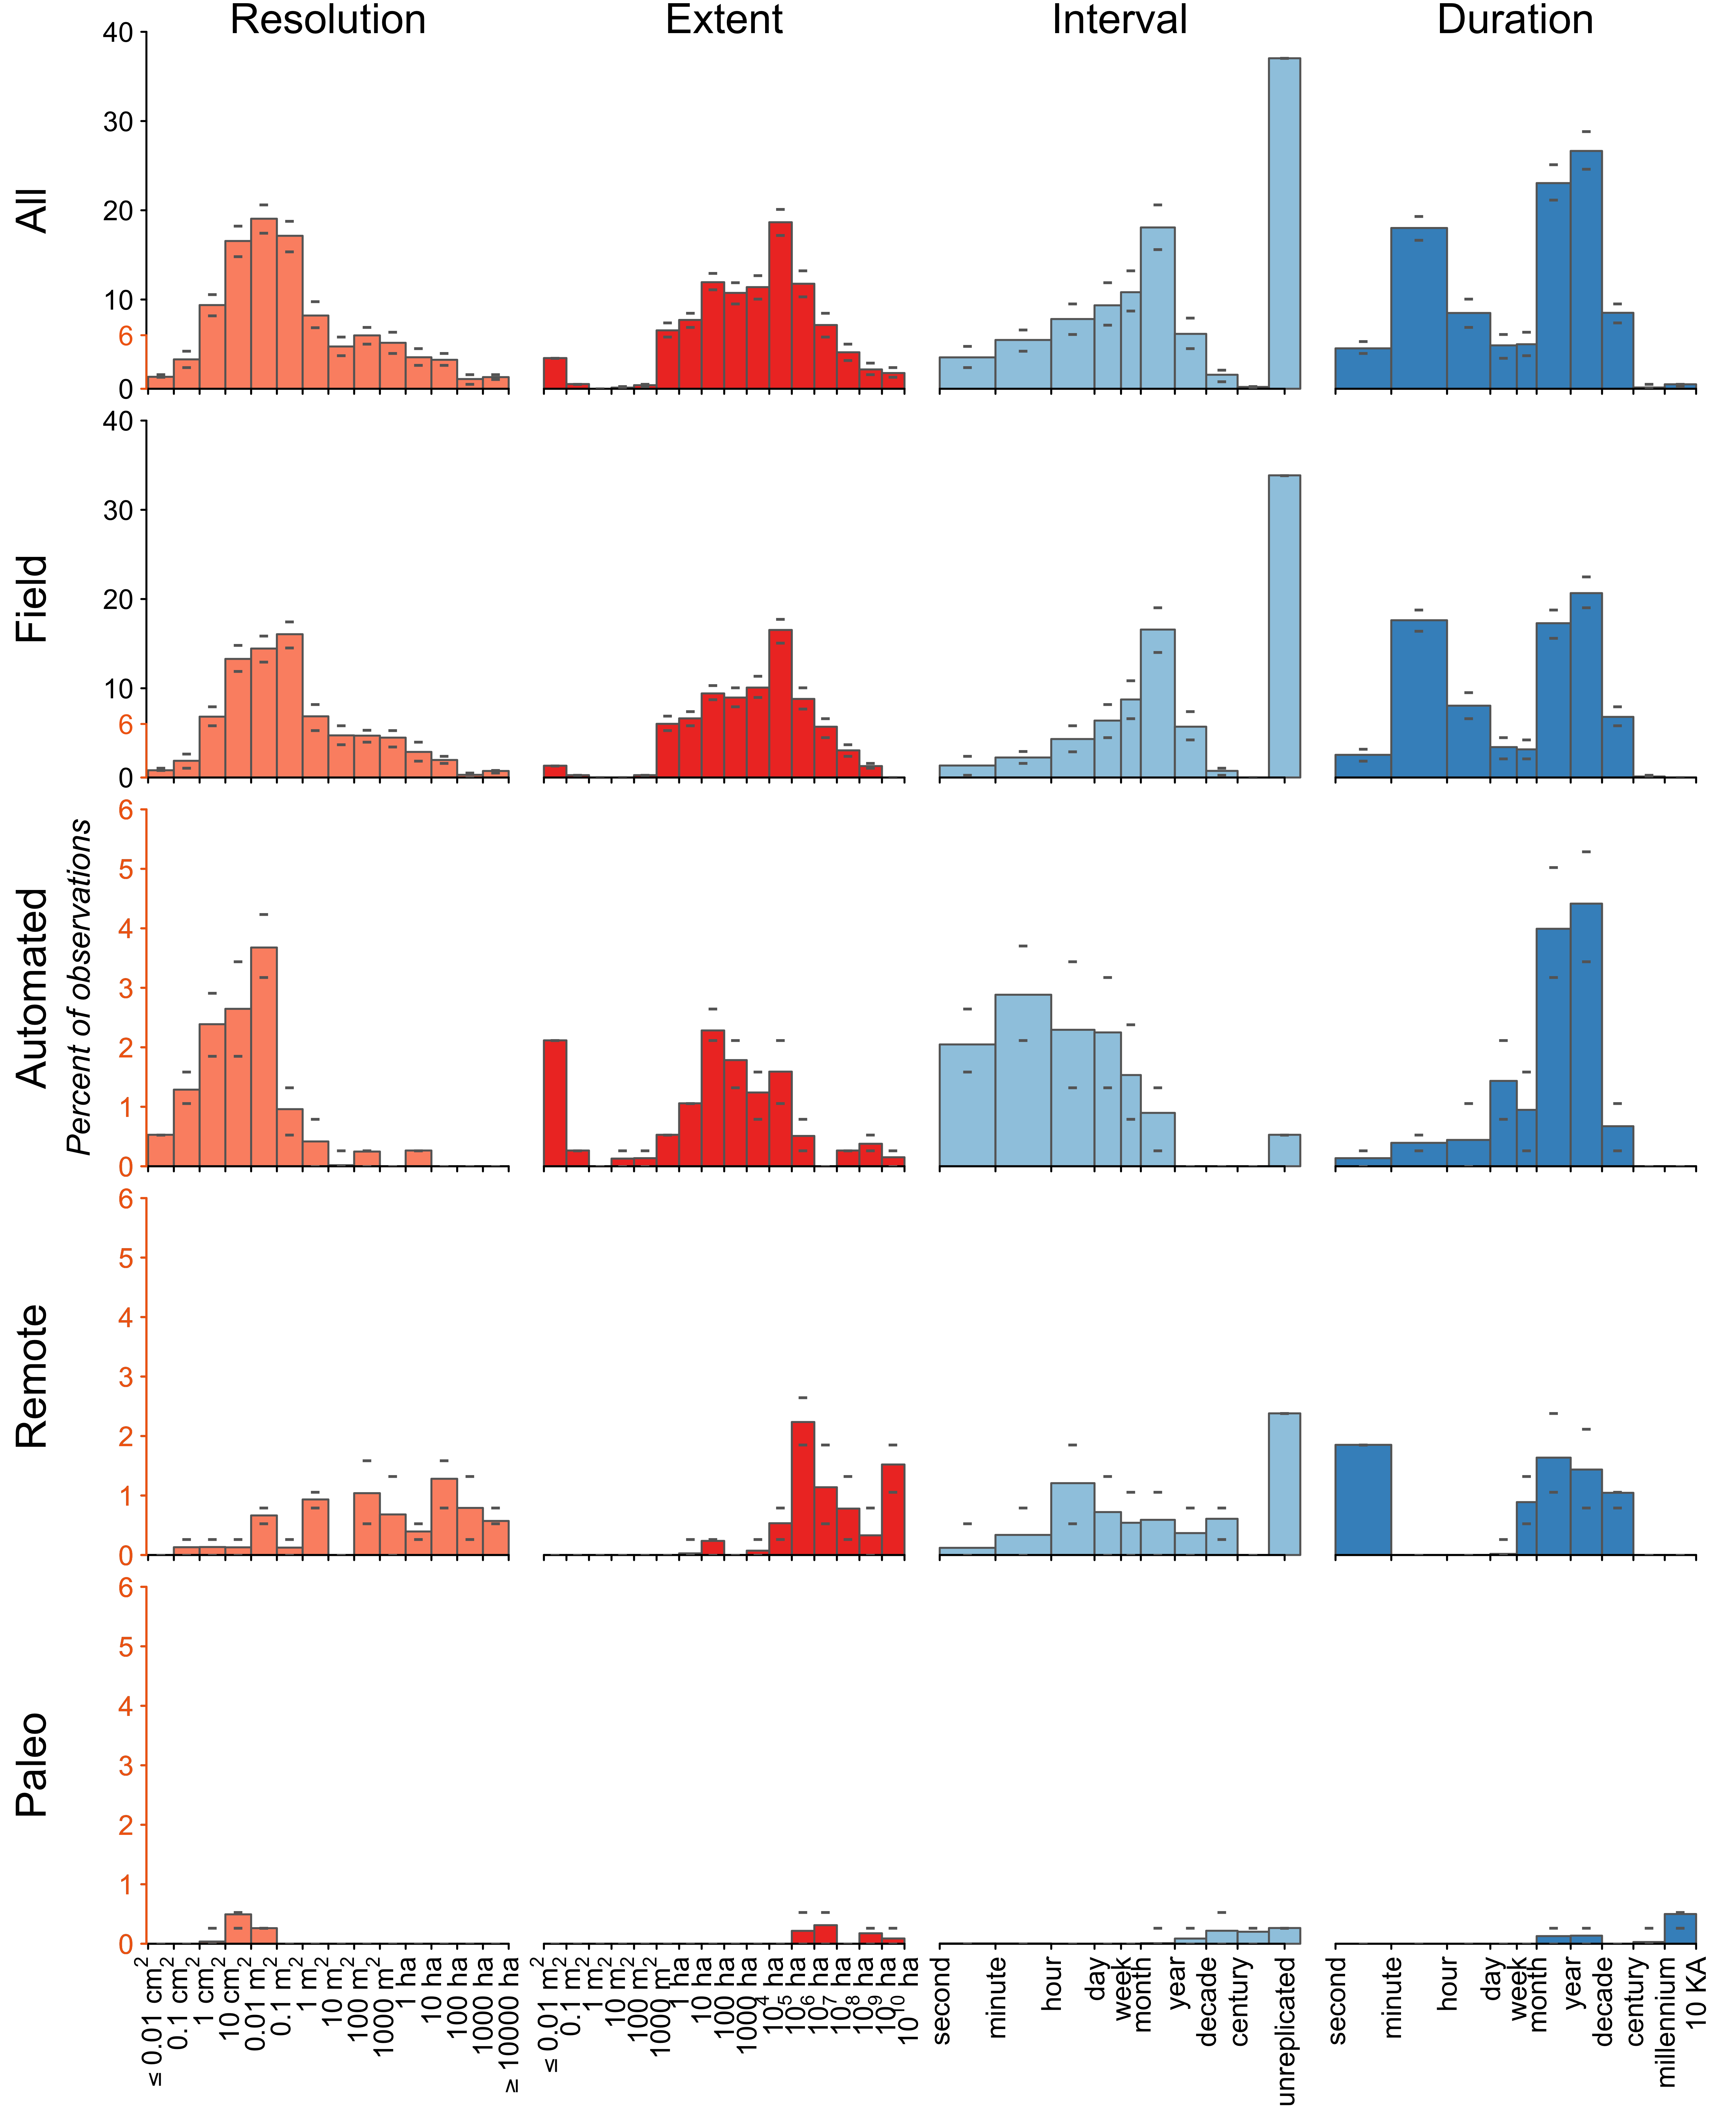
\includegraphics[width=0.9\textwidth]{../vignettes/figures/figS1.png}
\vspace{-5 pt}
\caption{Histograms of the resolution, extent, interval, and duration of observational scales, shown for all observational methods (top row) and for the four main observational methods (rows 2-5). Bars represent the average percentages for each bin realized after 1000 perturbed resamples, while grey bars indicate the 95\% confidence interval. Bar widths for interval and duration indicate differences in scale between x-axis labels. }
\label{obshists}
\end{figure}

\begin{figure}[!ht]
%\begin{wrapfigure}{c}{1\textwidth}
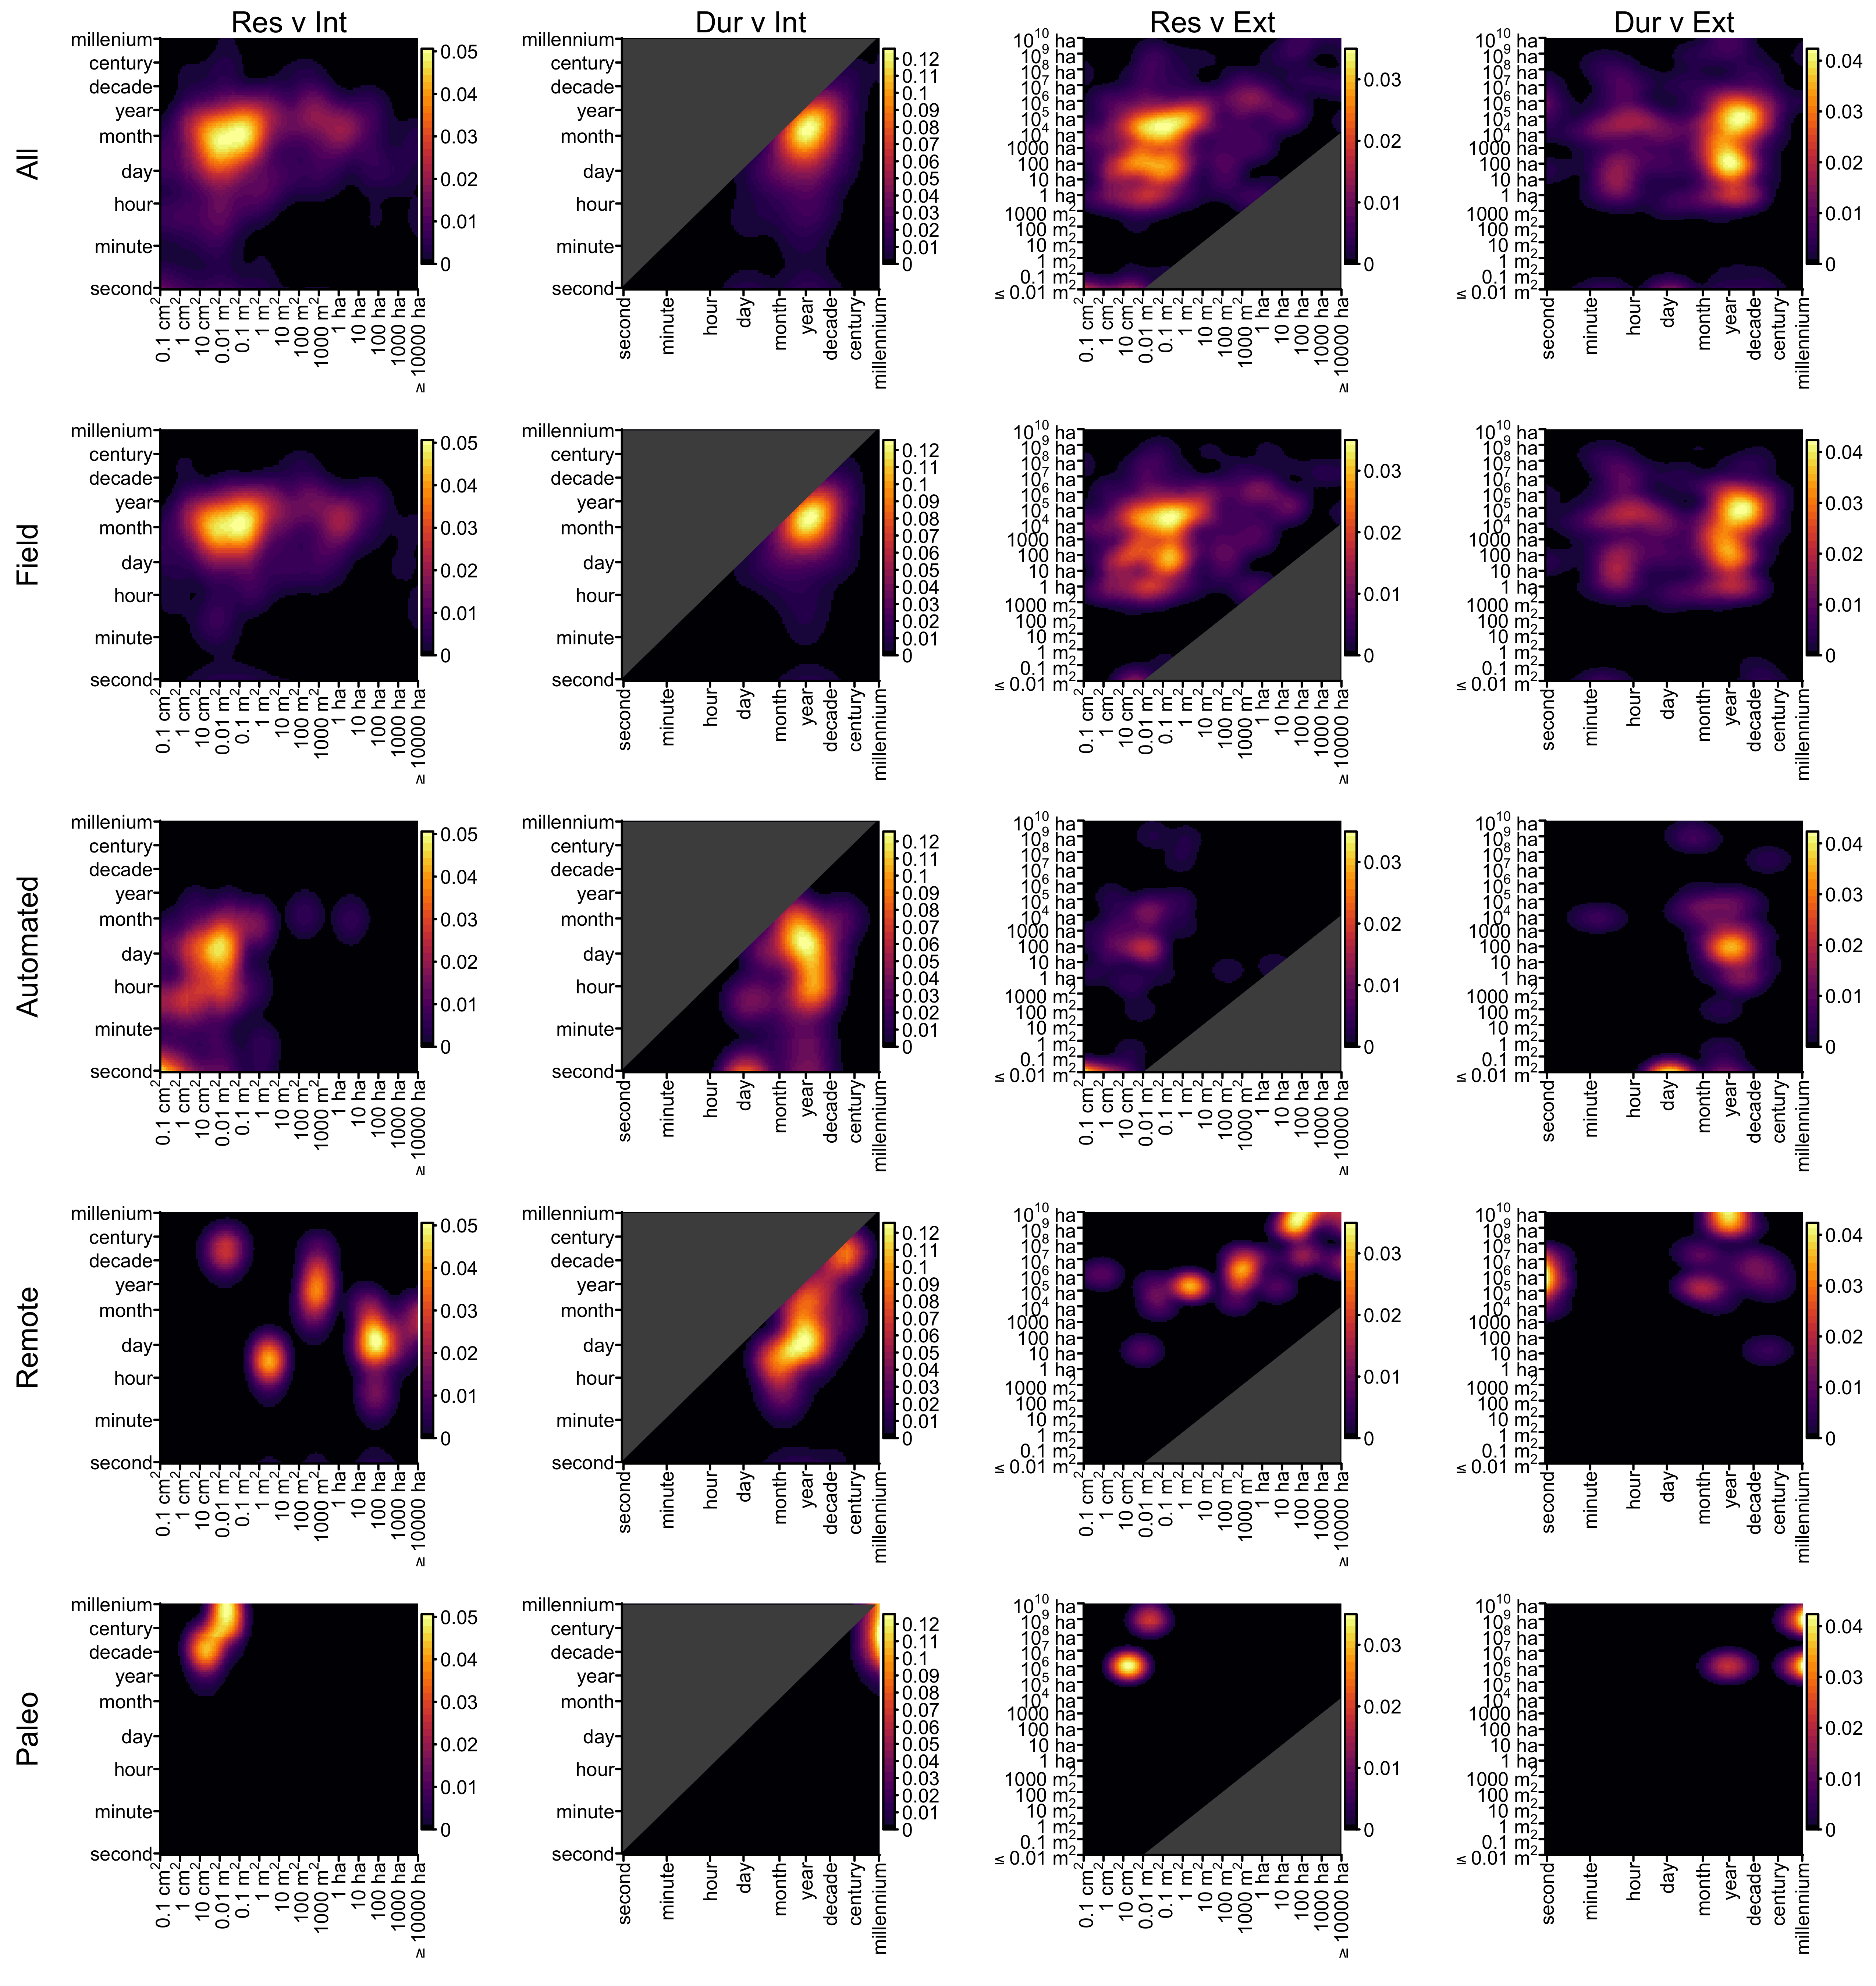
\includegraphics[width=1\textwidth]{../vignettes/figures/figS2.png}
\vspace{-20 pt}
\caption{Kernel density estimates across all observational methods (top row) and for each of the four primary observational methods (rows 2-5). Density estimates for resolution (x axis) versus interval (y axis) are presented in the first column, duration (x) versus interval (y) in the second column, resolution (x) versus extent (y) in the third column, and duration (x) versus extent (y) in the fourth column. Density estimates were applied to the log-transformed values of each observational dimension, and were rescaled to represent percentages. The grey shaded areas represent physically impossible domains (e.g. intervals greater than duration).}
\label{obskde}
\end{figure}

\begin{figure}[!ht]
%\begin{wrapfigure}{c}{1\textwidth}
\centering
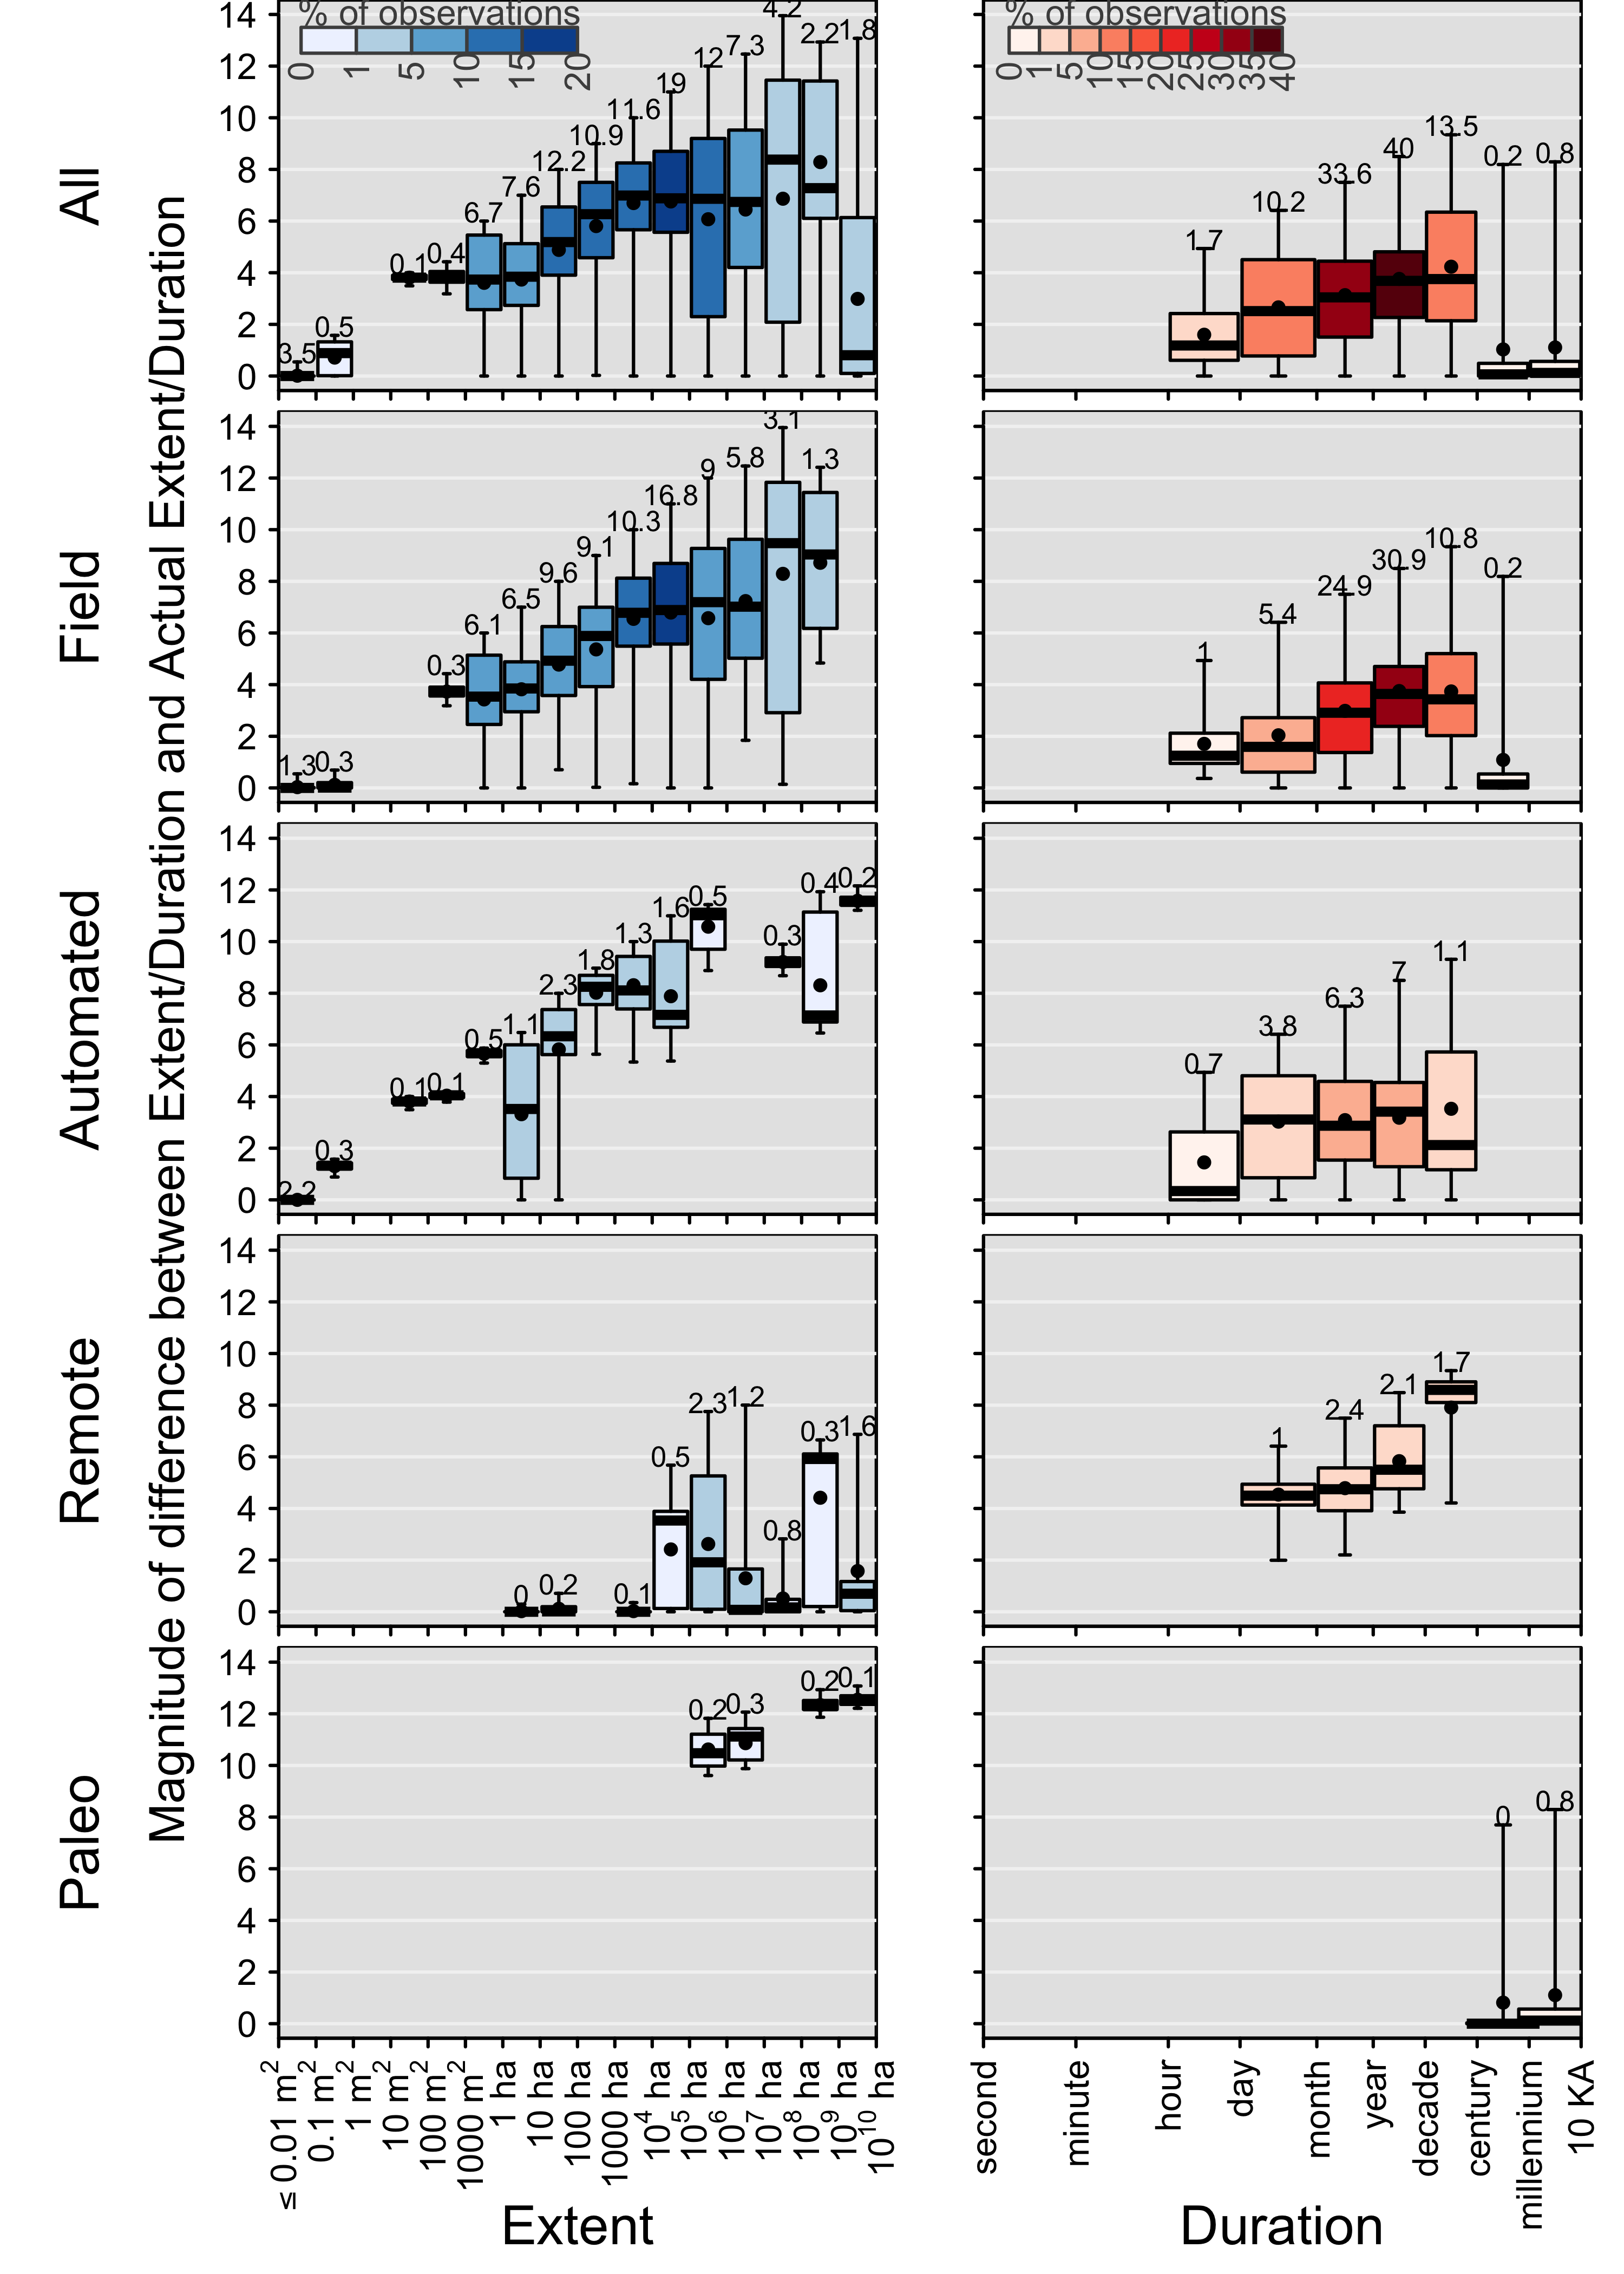
\includegraphics[width=0.7\textwidth]{../vignettes/figures/figS3.png}
\vspace{-5 pt}
\caption{The difference between extent and \emph{actual} extent and duration and \emph{actual} duration, as calculated across all observational methods (top row) and for each of the four primary observational methods. Difference values are expressed in terms of how many orders of magnitude larger (or longer) extent (duration) is than actual extent (actual duration), and are summarized (as box plots, with circle in box representing the mean and line the median) in bins representing increasing scales of actual extent/duration.  The percentages of observations falling within each bin are indicated by the color of the inter-quartile and the numeric value above the upper whisker.}
\label{obsdiff}
\end{figure}

\begin{figure}[!ht]
%\begin{wrapfigure}{c}{1\textwidth}
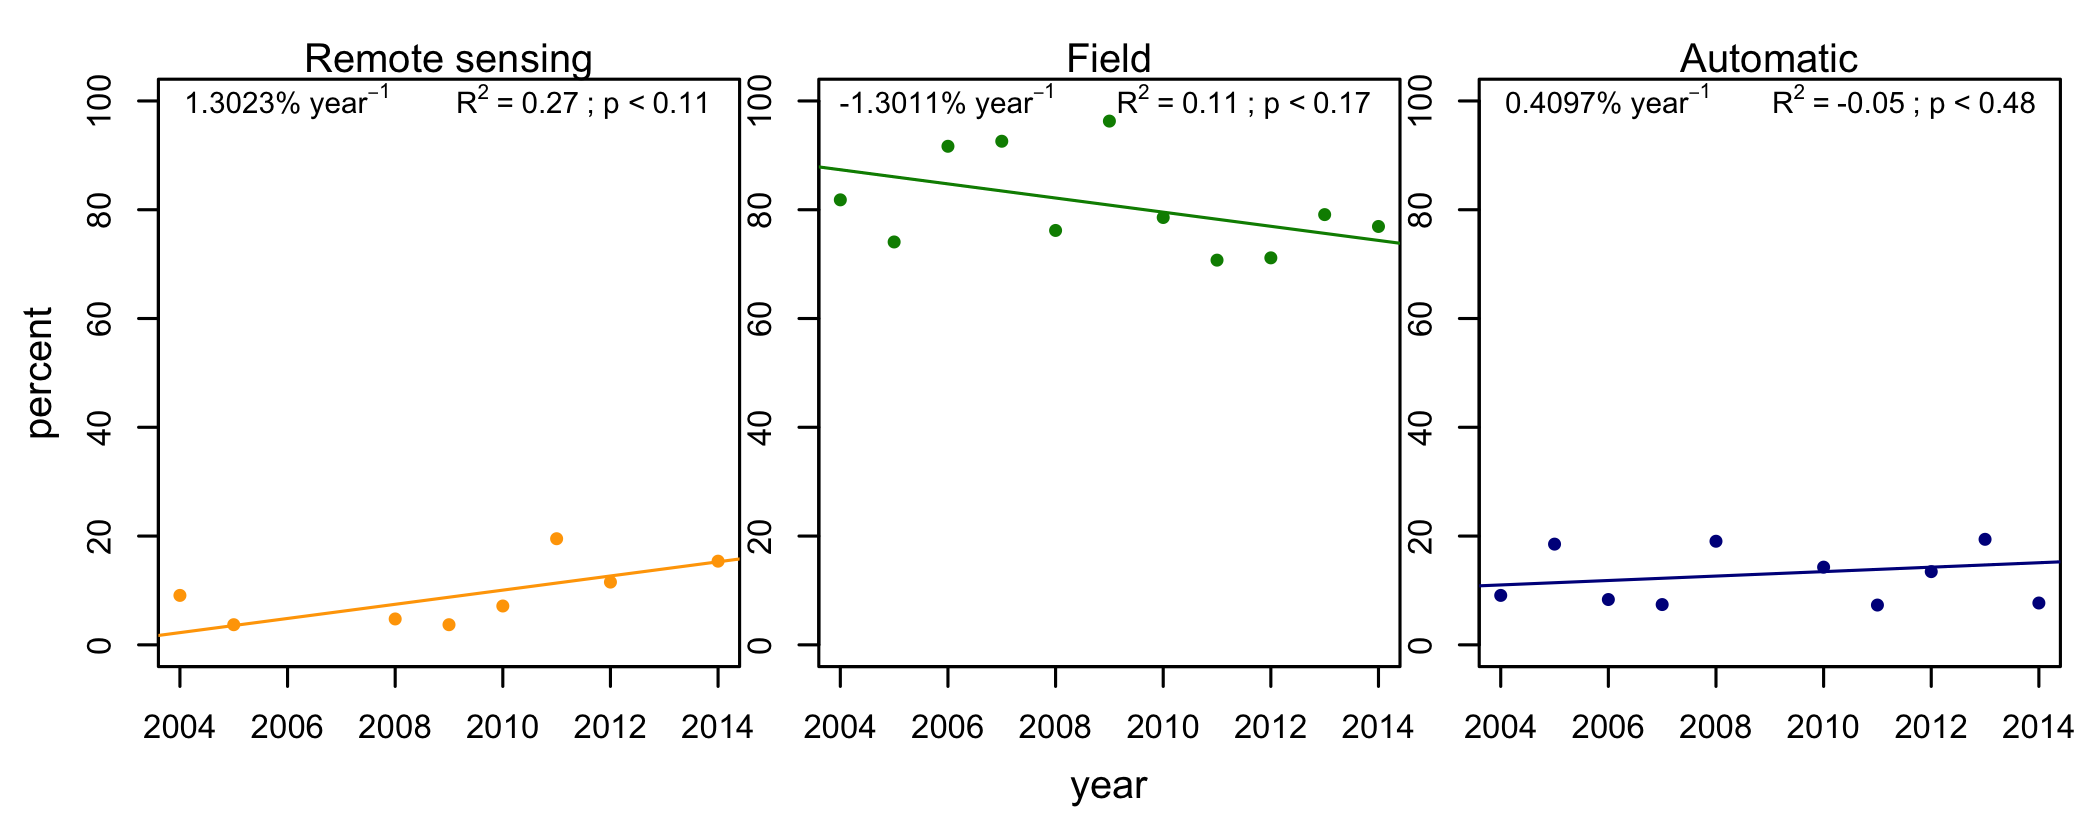
\includegraphics[width=1\textwidth]{../vignettes/figures/figS4.png}
\vspace{10 pt}
\caption{Trends in percentage of observing methods by year of publication. The coefficient of a weighted (by number of studies in each year) linear regression fit to the annual percentages of observations made with remote sensing (left), field methods (center), and automated sensors (right) is presented at the top of each plot, as well as the regression coefficient of determination and p-value. }
\label{type_by_yr}
\end{figure}

\begin{figure}[ht]
%\begin{wrapfigure}{c}{1\textwidth}
\center{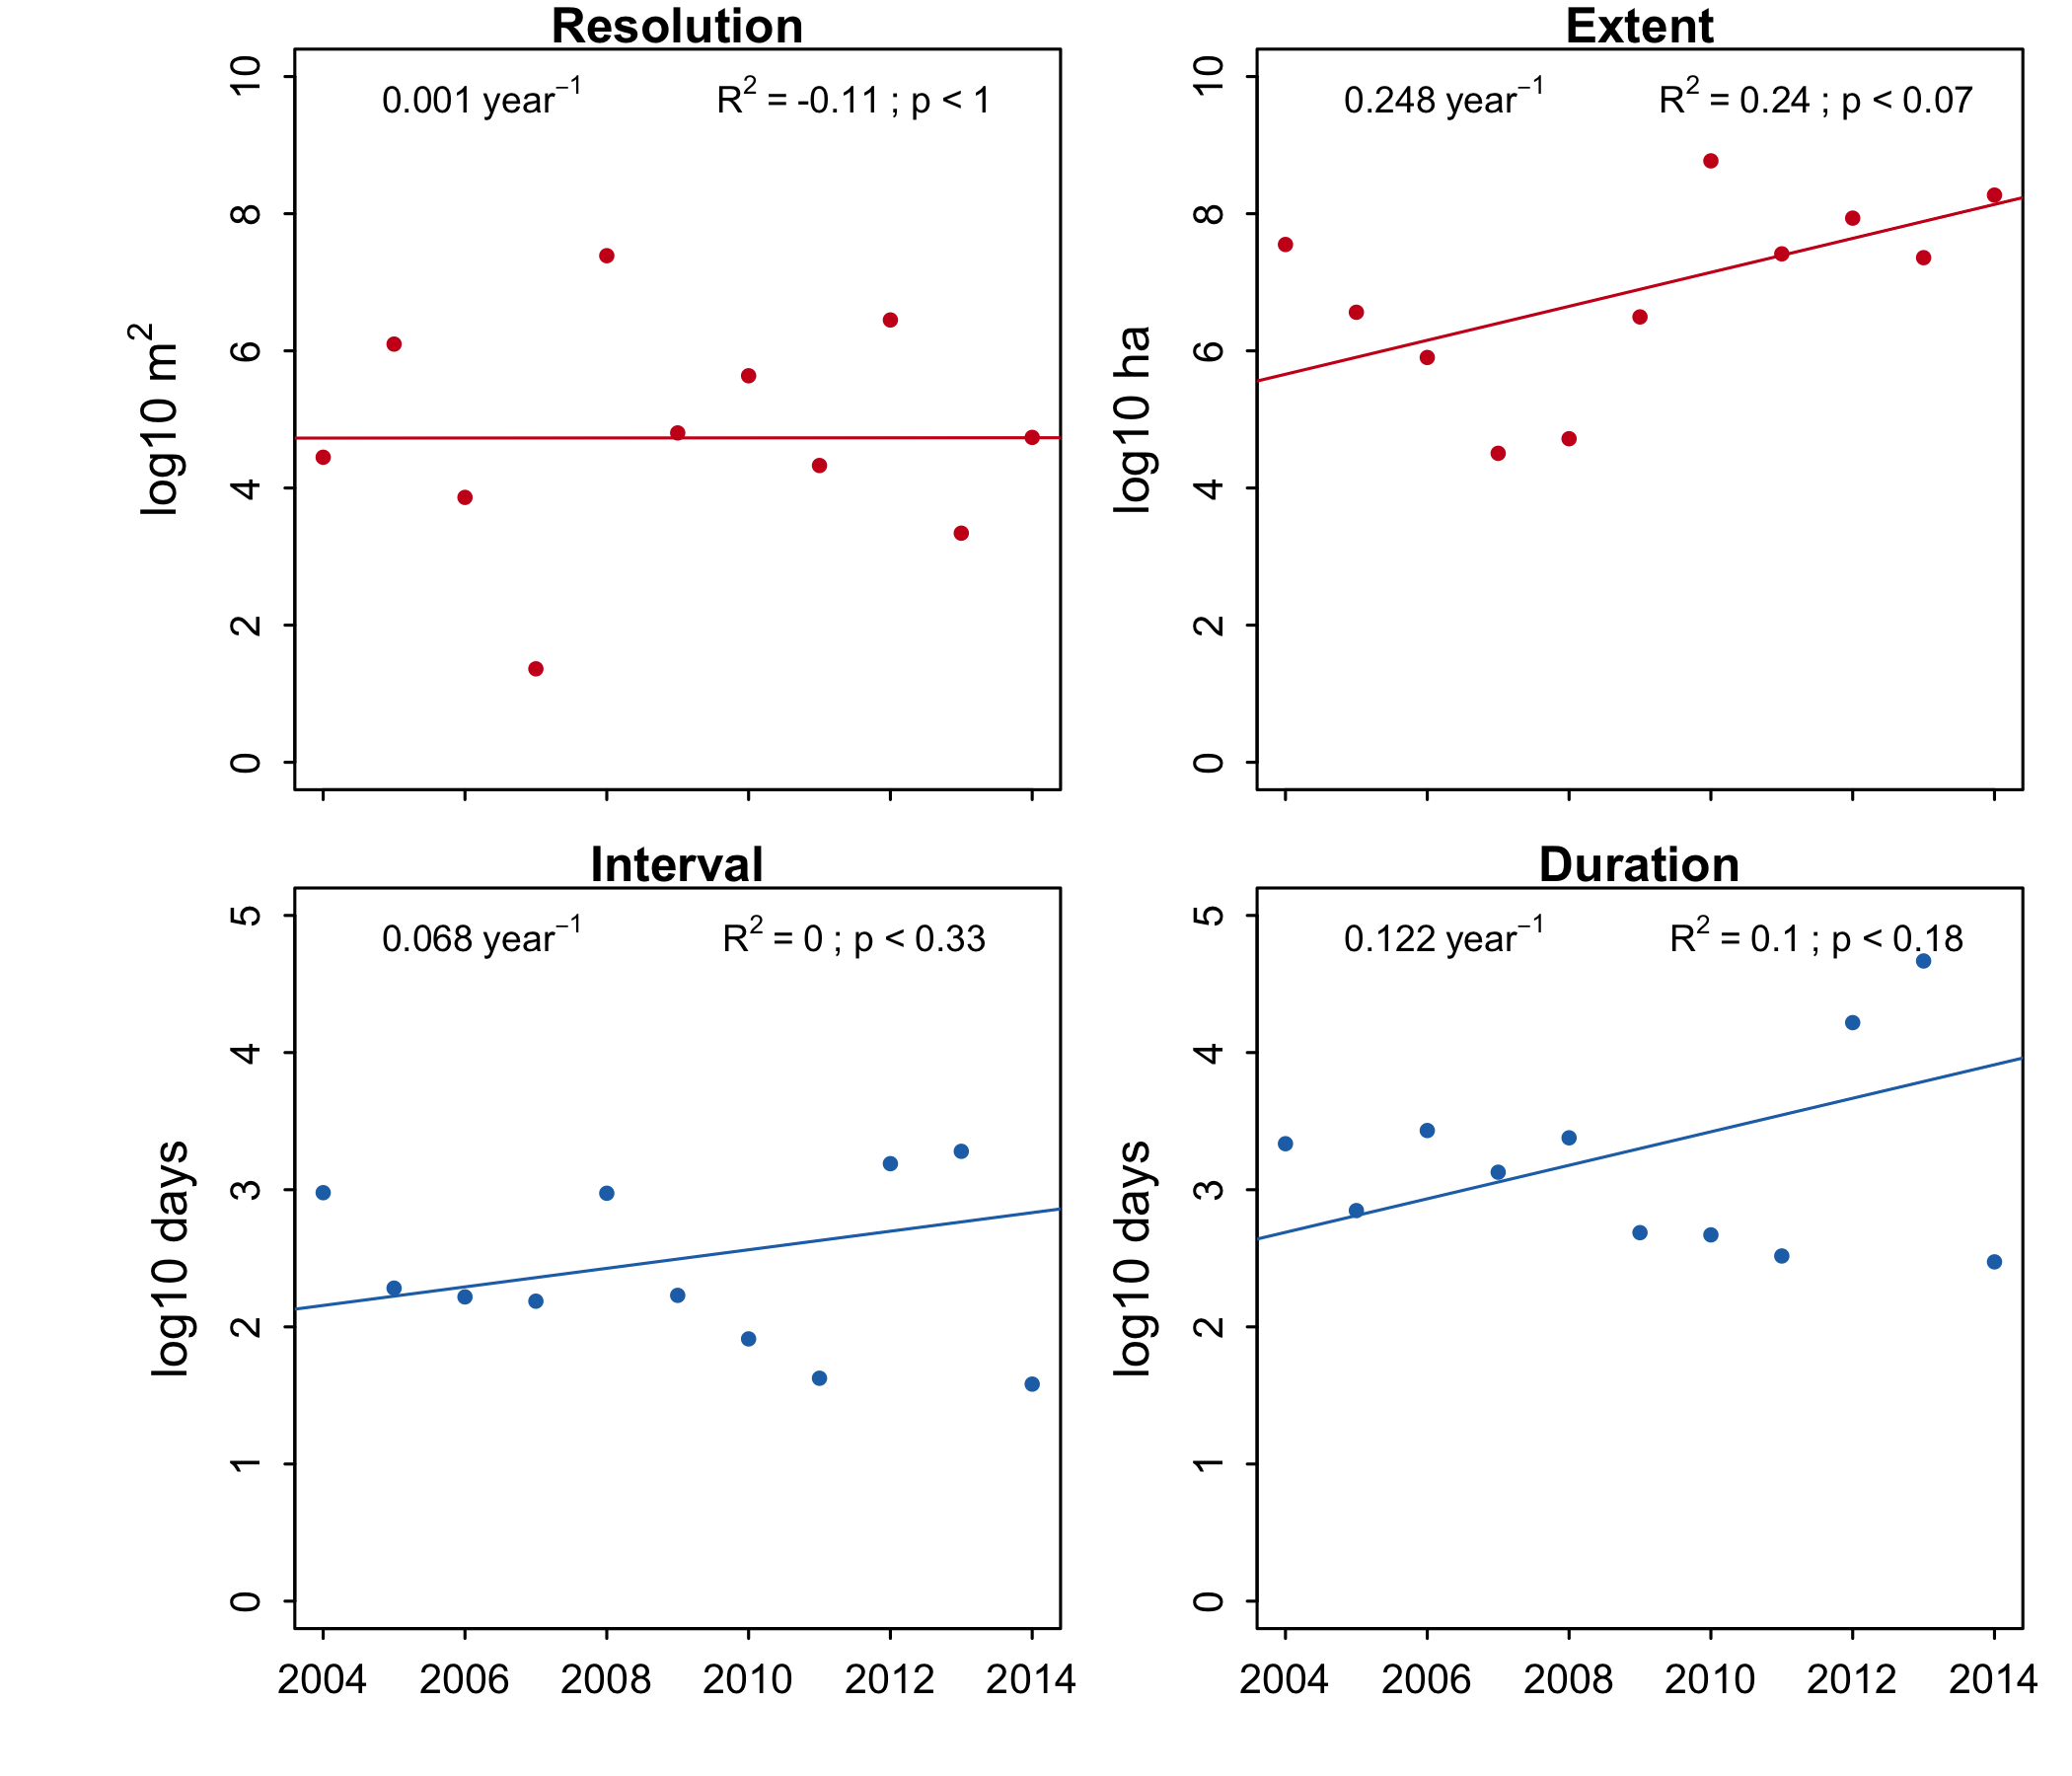
\includegraphics[width=0.8\textwidth]{../vignettes/figures/figS5.png}}
\vspace{5 pt}
\caption{Trends in observational scales by year of publication. The coefficient of a weighted (by number of studies in each year) linear regression, fit to the logarithm (base 10) of the mean scale values (calculated for each publication year) for the six assessed dimensions is presented at the top of each plot, as well as the model coefficient of determination and p-value. }
\label{sc_by_yr}
\end{figure}
%\clearpage

\begin{figure}[!ht]
%\begin{wrapfigure}{c}{1\textwidth}
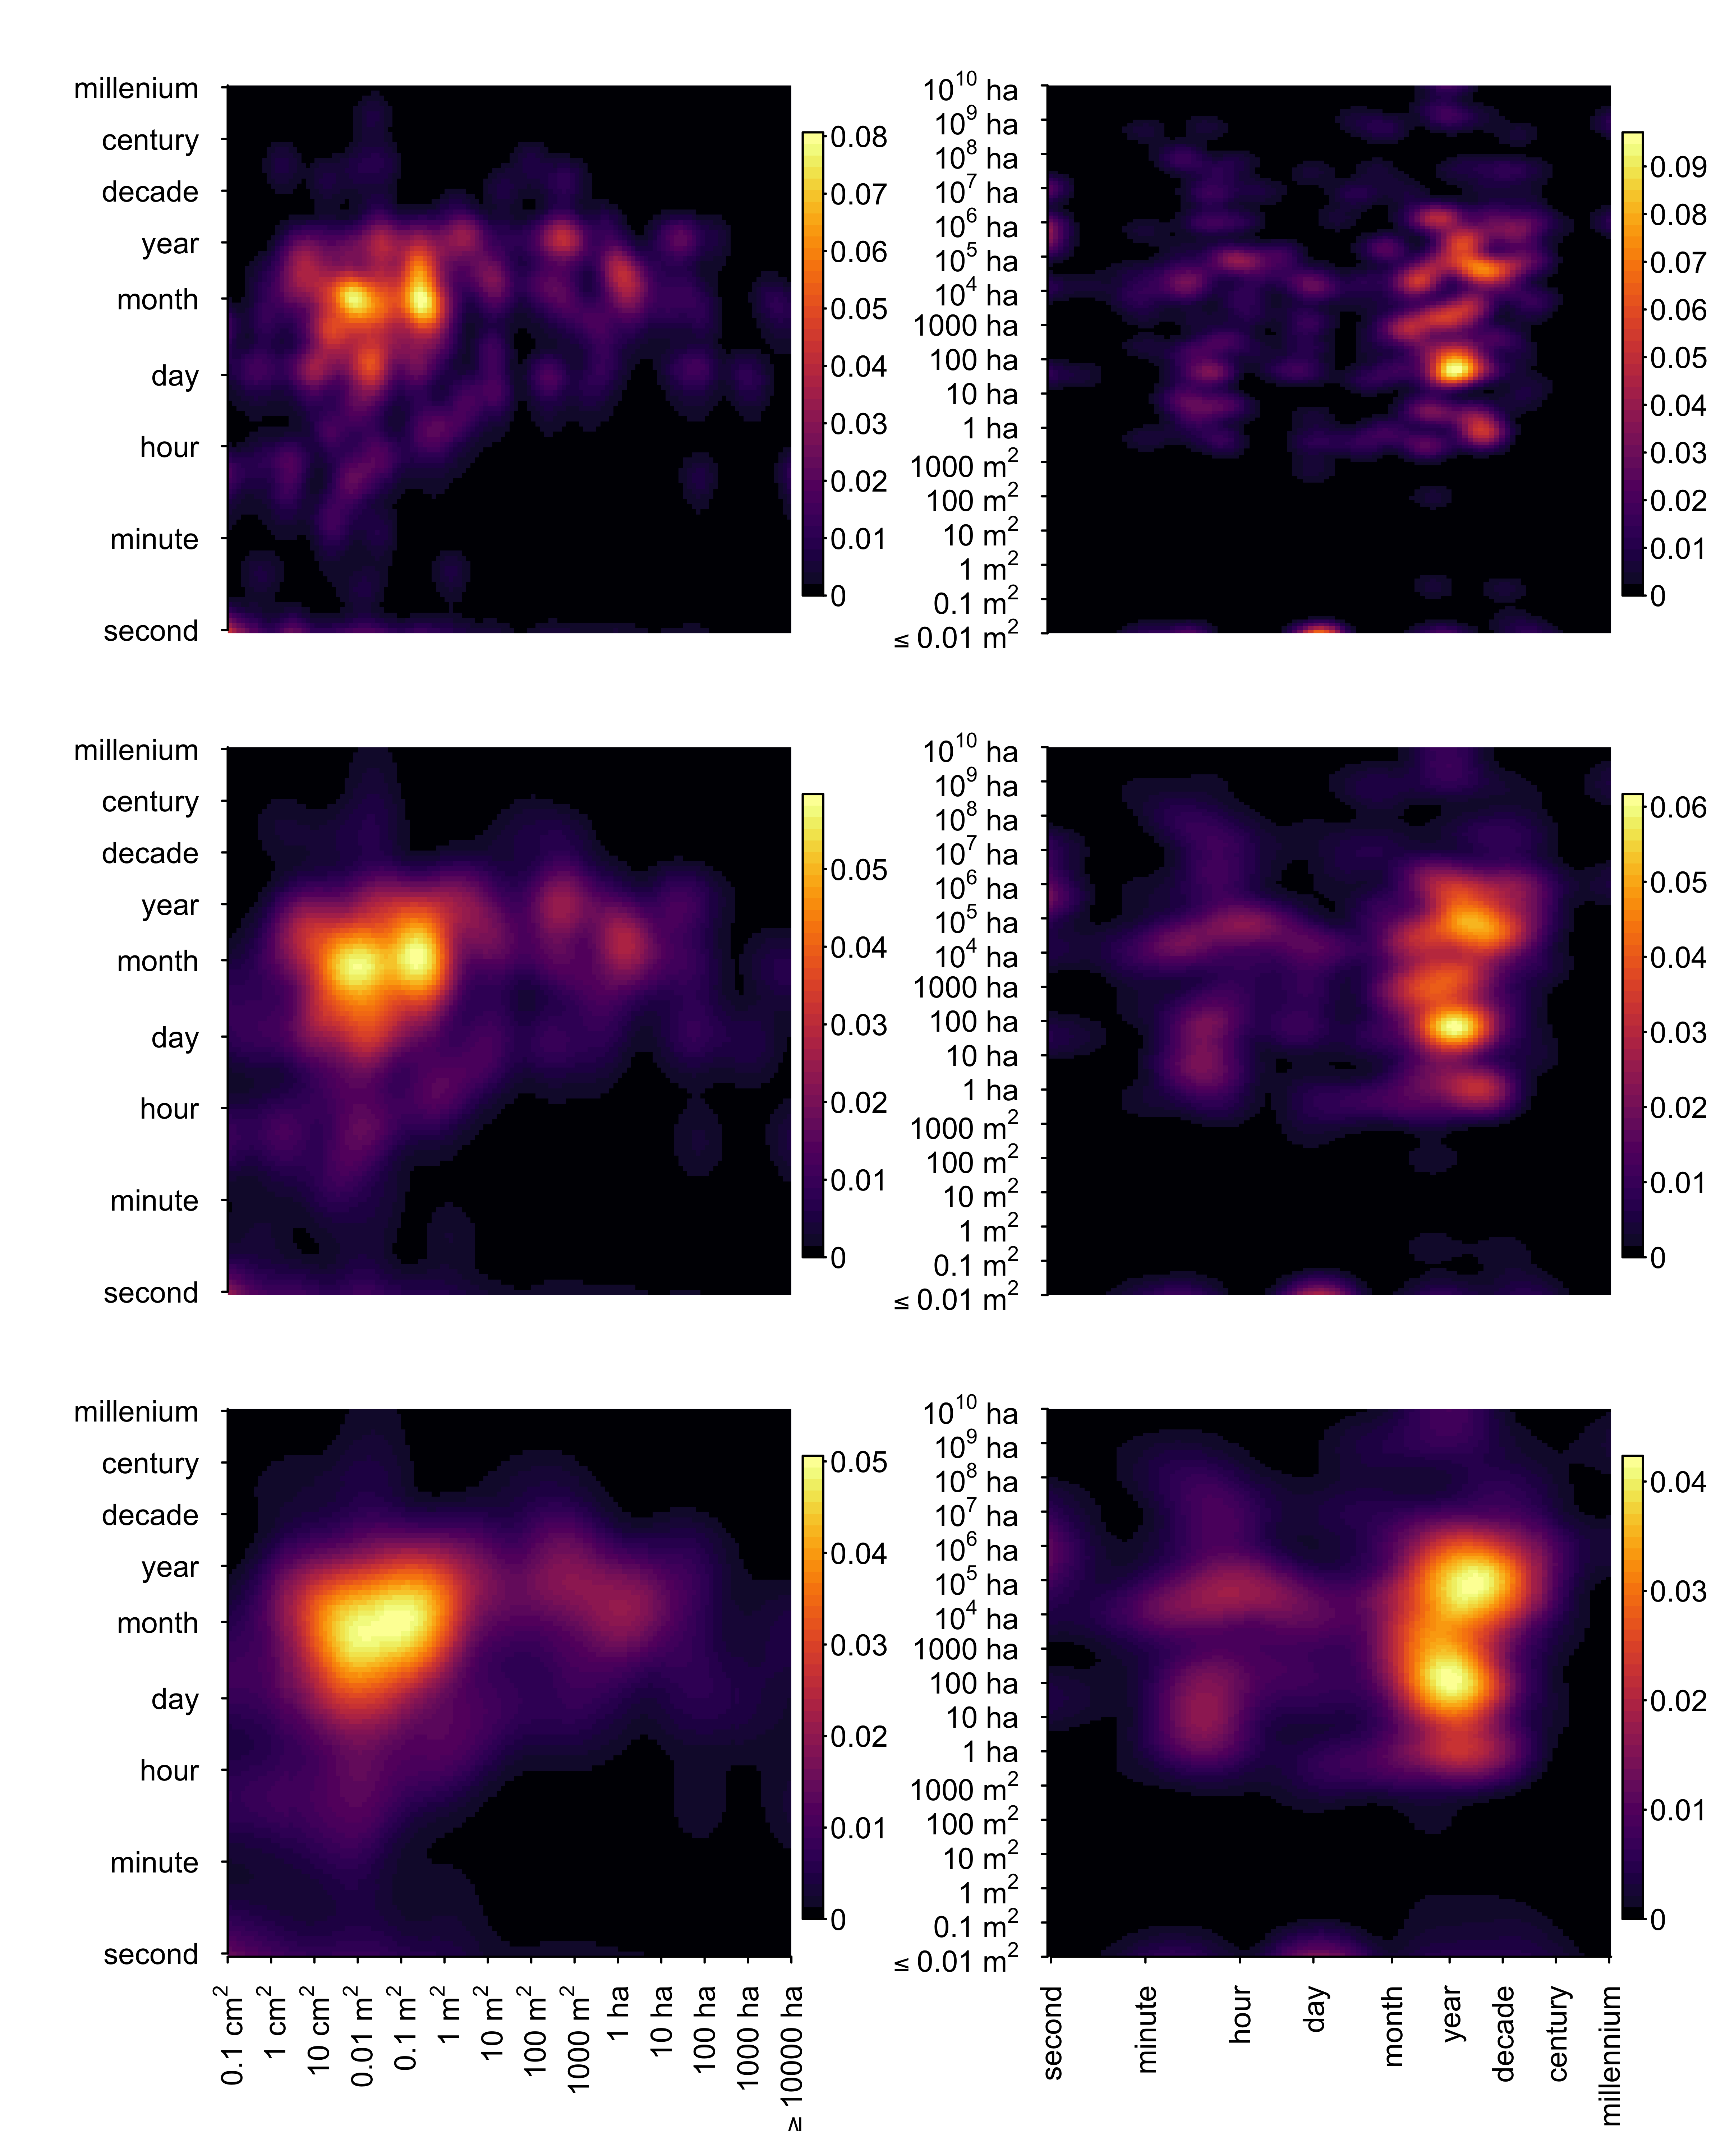
\includegraphics[width=0.9\textwidth]{../vignettes/figures/figS6.png}
\vspace{10 pt}
\caption{Two-dimensional kernel density estimates of observational densities within the domains defined by sampling interval and spatial resolution (left column) and duration and extent (right column), applied to log-transformed values of each observational dimension. Rows indicate the effects of selecting different bandwidths: 0.4 (top row); 0.7 (middle row); 1 (bottom row). }
\label{ksens}
\end{figure}
  
%\subsection*{Rationale}

%\begin{figure}[!ht]
%%\begin{wrapfigure}{c}{1\textwidth}
%\includegraphics[width=1\textwidth]{figures/hists.pdf}
%\vspace{-0.15 cm}
%\caption{Histograms of the spatial resolution (A) and extent (B), sampling interval (C) and temporal duration (D) of ecological observations collected from the surveyed ecological studies. Bars represent percentage of the 367 collected records falling within each bin.}
%\label{afoto1}
%\end{figure}

\clearpage
\bibliography{/Users/lestes/Dropbox/publications/fullbib}

\bibliographystyle{naturemag}

\end{document}




















